\documentclass[11pt]{article}

\usepackage[margin=1in]{geometry}
\usepackage{amsmath,amssymb,amsthm}
\usepackage{graphicx}
\usepackage{booktabs}
\usepackage{xcolor}
\usepackage[numbers,sort&compress]{natbib}
\usepackage[colorlinks=true,linkcolor=black,citecolor=blue,urlcolor=blue]{hyperref}

\graphicspath{{figures/}}
\newcommand{\sr}{\mathrm{SR}}
\newcommand{\theyll}{\theta}

\title{\bfseries Plateaus, Peaks, and the Probability of Backtest Overfitting:\\
A Controlled Validation of Parameter-Robustness Heuristics}

\author{Eugen Soloviov\thanks{Independent Researcher. ORCID:
\href{https://orcid.org/0009-0006-3148-111X}{0009-0006-3148-111X}.
Correspondence: \href{mailto:suenot@gmail.com}{suenot@gmail.com}.
Code to reproduce every number and figure:
\url{https://github.com/suenot/plateau-robustness}.}}

\date{}

\begin{document}
\maketitle

\begin{abstract}
Practitioners optimizing trading-strategy hyperparameters are widely advised to
prefer a \emph{plateau}---a broad region of consistently good performance---over
a \emph{sharp peak}, on the grounds that peaks are artifacts of in-sample noise.
This ``parameter-robustness'' heuristic is folklore in the algorithmic-trading
literature, yet it has never been validated against ground truth or compared to
formal backtest-overfitting diagnostics. We build a controlled simulation in
which the population Sharpe surface over the hyperparameter grid is known, draw
independent in-sample and out-of-sample (OOS) returns with realistic
cross-strategy correlation, and evaluate on the same data: (i) local
plateau-geometry metrics (relative plateau width, sensitivity, a combined
robustness score, and a top-versus-typical ``outlier gap''), measured on a
kernel-smoothed surrogate of the in-sample landscape; (ii) the Probability of
Backtest Overfitting (PBO); and (iii) the Probabilistic and Deflated Sharpe
Ratios (PSR, DSR). Across $9{,}000$ simulated optimization problems the
plateau-\emph{shape} metrics are weak standalone diagnostics, and the popular
fixed thresholds (e.g.\ ``robustness score $>0.1$'') are not calibrated. The
strongest single diagnostic is the plain PSR against zero skill---the
significance test, not the multiplicity deflation, carries the signal in this
setting. Geometry still adds information where it has any: combining shape
metrics with the statistical diagnostics significantly improves detection of
the sharp-peak (\emph{fragile}) mode and of every mode in two dimensions, but
is statistically indistinguishable from the plain PSR for no-edge detection in
one dimension. As a \emph{selection principle}, however, the heuristic works
outright: choosing the optimum of the smoothed surrogate instead of the raw
argmax raises OOS Sharpe by $0.12$ on average in one dimension and $0.31$ in
two, with a gain that is positive in every curvature tercile and increases
monotonically with the curvature of the surrogate landscape at its optimum. We
conclude that ``prefer plateaus'' is sound as a selection bias---increasingly so
as the number of parameters grows---but unreliable as a standalone overfitting
test, and should be used alongside, not instead of, statistical significance
controls.
\end{abstract}

\section{Introduction}

Optimizing the free parameters of a trading strategy on historical data is an
invitation to overfit. With enough configurations tried, some will look
excellent in sample purely by chance and collapse out of sample
\citep{bailey2017pbo,harvey2016crosssection,lopezdeprado2018}. The standard
statistical responses correct the \emph{selected} performance for the number of
trials and for non-normality---the Deflated Sharpe Ratio (DSR)
\citep{bailey2014dsr}, the Probability of Backtest Overfitting (PBO)
\citep{bailey2017pbo}, and data-snooping reality checks
\citep{white2000reality,harvey2015backtesting}.

A second, more geometric piece of advice circulates widely in practitioner
writing \citep{pardo2008,lopezdeprado2018,arnott2019protocol}: do not just take
the best parameter set, look at the \emph{shape} of the objective around it. A
broad ``plateau'' of similar performance is presumed robust; a narrow ``peak''
that collapses one grid step away is presumed to be fitted noise. The intuition
mirrors the flat-minima literature in machine learning, where wide minima are
argued to generalize better than sharp ones
\citep{hochreiter1997flat,keskar2017sharp}. Modern hyperparameter tooling makes
the geometry easy to inspect---slice plots, contour heatmaps, and functional
ANOVA importances \citep{hutter2014fanova,akiba2019optuna}---and several authors
propose scalar ``plateau metrics'' (sensitivity ratios, plateau widths,
robustness scores) to formalize it.\footnote{The specific scalar metrics we
validate---robustness score, plateau width, sensitivity, and the
top-versus-typical outlier check---follow the author's earlier practitioner
article \citep{soloviov2026plateau}, where they were proposed without
ground-truth validation; the present paper subjects them to their first
controlled test.}

Despite its popularity, the plateau heuristic has, to our knowledge, never been
tested where the truth is known. Does plateau geometry actually predict
out-of-sample degradation? Are the proposed scalar metrics and their thresholds
meaningful? How do they compare to, and combine with, the statistical diagnostics
designed for the same problem? We answer these questions in a controlled
simulation and report results that are useful precisely because they are mixed.

\paragraph{Contributions.}
\begin{enumerate}\itemsep2pt
\item A reproducible simulation framework in which the population Sharpe surface
over a hyperparameter grid is known, so selection quality, in-sample inflation,
and out-of-sample performance are all measurable ground truth
(Section~\ref{sec:framework}).
\item A head-to-head evaluation of the plateau metrics against PBO, DSR, and the
plain probabilistic Sharpe ratio (PSR) as overfitting \emph{classifiers}, with
bootstrap confidence intervals. The shape metrics are weak alone (no-edge ROC
AUC $0.501$ in one dimension, i.e.\ chance); the strongest single diagnostic is
the PSR against zero skill (AUC $0.808$), ahead of the DSR ($0.785$) and PBO
($0.669$), and the article-style fixed thresholds do not correspond to
calibrated decision boundaries (Section~\ref{sec:diagnostic}).
\item Evidence that geometry and statistics detect \emph{different} overfitting
modes, so that a combined classifier significantly improves detection of the
sharp-peak \emph{fragile} mode---and of every mode in two dimensions---while
adding nothing significant over the plain PSR for no-edge detection in one
dimension (Sections~\ref{sec:complementarity}--\ref{sec:dimension}). We also
show the geometry must be \emph{anchored at the surrogate optimum}: measured at
the naive argmax instead, the same metrics become anti-informative
(Section~\ref{sec:anchoring}).
\item A demonstration that, as a \emph{selection rule}, preferring the broad
optimum of a denoised landscape delivers a real out-of-sample gain that is
positive in every curvature tercile, grows with the sharpness of the surrogate
optimum and with dimensionality, and depends on the surrogate bandwidth in a
disclosed way (Section~\ref{sec:selection}).
\end{enumerate}

\section{Background and metrics}
\label{sec:background}

\paragraph{Setting.} A strategy is evaluated at configurations $\theyll$ on a
grid $\Theta \subset [0,1]^d$. Each configuration produces a return series; over a
sample of $T$ periods its annualized Sharpe ratio is estimated as
$\widehat{\sr}(\theyll) = \bar r(\theyll)/s(\theyll)\sqrt{P}$ with $P=252$. The
optimizer reports $\hat\theyll = \arg\max_{\theyll} \widehat{\sr}_{\text{IS}}(\theyll)$;
the quantity that matters is the realized out-of-sample $\sr_{\text{OOS}}(\hat\theyll)$.

\paragraph{Plateau metrics.} We study the local-geometry metrics of the
practitioner tradition, computed from the in-sample Sharpe landscape, fixing
estimator flaws we observed in circulating implementations. First, per-parameter
quantities are taken along the axis through the optimum with the other
parameters \emph{held fixed} (exact on a grid), rather than by regressing over
top trials in which all parameters co-vary. Second, the plateau width is the
\emph{connected} super-level set around the optimum, not $\max-\min$ over all
``good'' points, which a single distant lucky point inflates.

For axis $i$, with optimum value $\sr^\star$ and margin $\delta$ (in Sharpe
units), the \emph{relative plateau width} is
\begin{equation}
W_i \;=\; \frac{\big|\{\,\text{contiguous run through }\hat\theyll : \widehat{\sr}(\theyll)\ge \sr^\star-\delta\,\}\big|}{\text{axis length}} \in [0,1].
\end{equation}
The \emph{sensitivity} is the Sharpe drop when stepping a fixed fraction of the
axis away from the optimum (well defined for any sign of $\sr^\star$, unlike the
elasticity used in some sources, whose first-derivative term vanishes at an
interior maximum). The \emph{robustness score} aggregates widths with
first-order functional-ANOVA weights $w_i$ \citep{hutter2014fanova}:
\begin{equation}
R \;=\; \prod_{i=1}^{d} W_i^{\,w_i}, \qquad \textstyle\sum_i w_i = 1 .
\label{eq:R}
\end{equation}
A high $R$ is meant to signal robustness; a common rule of thumb labels $R>0.1$
``robust'' and $R<0.01$ ``overfit.'' Note that in $d{=}1$ there is a single
axis with unit weight, so $R \equiv W_1$: the robustness score and the plateau
width coincide by construction. Finally, the \emph{outlier gap} asks whether the
best few cells are outliers relative to typical performance:
$G = \mathrm{mean}\big(\text{top-3 } \widehat{\sr}\big) - \mathrm{median}\big(\widehat{\sr}\big)$.
The practitioner version is the \emph{ratio} of top-3 to median, which is
ill-posed whenever the median Sharpe is near zero or negative---exactly the
no-edge landscapes that matter most; the difference form preserves the intent
and is well defined everywhere.

\paragraph{Statistical baselines.} We compare against three standard
diagnostics computed on the same returns. The \emph{Probability of Backtest
Overfitting} \citep{bailey2017pbo} uses combinatorially-symmetric
cross-validation (CSCV): the $T$ observations are split into $S$ blocks; over
all $\binom{S}{S/2}$ train/test partitions one records the relative
out-of-sample rank of the in-sample-best strategy, and PBO is the fraction of
partitions in which that rank falls below the median. The \emph{probabilistic
Sharpe ratio} \citep{bailey2012psr} $\mathrm{PSR}(\sr^{*})$ is the probability
that the true Sharpe exceeds a benchmark $\sr^{*}$, given the sample length,
skewness, and kurtosis of the selected strategy's returns; $\mathrm{PSR}(0)$
tests significance against zero skill with \emph{no} multiplicity correction.
The \emph{Deflated Sharpe Ratio} \citep{bailey2014dsr} is
$\mathrm{PSR}(\sr_0)$ with the benchmark set to the expected maximum Sharpe of
$N$ independent null trials,
\begin{equation}
\sr_0 \;=\; \sqrt{V}\Big[(1-\gamma)\,\Phi^{-1}\!\big(1-\tfrac1N\big) + \gamma\,\Phi^{-1}\!\big(1-\tfrac1{Ne}\big)\Big],
\end{equation}
where $V$ is the cross-trial variance of the Sharpe estimates and $\gamma$ is the
Euler--Mascheroni constant; a low DSR flags a selection that is not significant
once the number of trials and non-normality are accounted for. We set $N$ to
the full grid size ($41$ in $d{=}1$, $1681$ in $d{=}2$). This follows common
practice but overstates the effective number of trials: grid trials are strongly
correlated (a shared market factor plus a smooth true surface), and
\citet{bailey2014dsr} prescribe the number of \emph{effectively independent}
trials. We disclose this choice and report a sensitivity check in
Section~\ref{sec:diagnostic}.

\section{Simulation framework}
\label{sec:framework}

We treat backtest optimization as selecting from a grid of noisy estimates of a
known surface. The \emph{population} annualized-Sharpe surface
$\sr_{\text{true}}(\theyll)$ is a sum of a broad Gaussian bump (the plateau) and
an optional narrow Gaussian bump (the spike), on a floor $\mu_0$:
\begin{equation}
\sr_{\text{true}}(\theyll) = \mu_0 + A_p \exp\!\Big(\!-\tfrac{\|\theyll-c_p\|^2}{2\ell_p^2}\Big)
+ A_s \exp\!\Big(\!-\tfrac{\|\theyll-c_s\|^2}{2\ell_s^2}\Big).
\end{equation}
Each configuration emits per-period returns
$r_t(\theyll) = \sr_{\text{true}}(\theyll)/\sqrt{P} + \sqrt{c}\,F_t + \sqrt{1-c}\,\varepsilon_t(\theyll)$,
with a shared market factor $F_t$ and idiosyncratic $\varepsilon$, both standard
normal; the factor share $c$ equals the cross-strategy correlation and is the
structure PBO and DSR are designed for. We draw independent in-sample
($T_{\text{IS}}\in\{120,252,504\}$) and out-of-sample ($T_{\text{OOS}}=504$)
blocks.

\paragraph{Surrogate.} At $T_{\text{IS}}=252$ the per-configuration Sharpe
estimate has noise of order $1.0$ annualized, so the \emph{raw} per-cell surface
is dominated by noise and any argmax looks like a needle. Practitioners never
read raw per-point values; they assess the landscape through a surrogate---the
smoothing implicit in contour plots and functional ANOVA. We model that surrogate
with a Gaussian kernel of disclosed bandwidth and compute all plateau
geometry on it (Figure~\ref{fig:setup}). The statistical baselines act on the raw
returns, as their definitions require. Boundary handling matters more than one
might expect: padding the convolution by replicating edge values concentrates
roughly half the kernel mass onto a single boundary cell, inflating its noise
variance; in a flat-null check, $39.9\%$ of surrogate argmaxes then land in the
outer three cells per side, versus $14.6\%$ under uniformity. We therefore use
mask-normalized smoothing (zero-padded convolution divided by the convolution of
a ones mask), which removes the weighting artifact; the residual edge share
($29.7\%$ in the same check) reflects the genuinely higher estimation variance
where fewer neighbors are observed, not a weighting bias.

\begin{figure}[t]
\centering
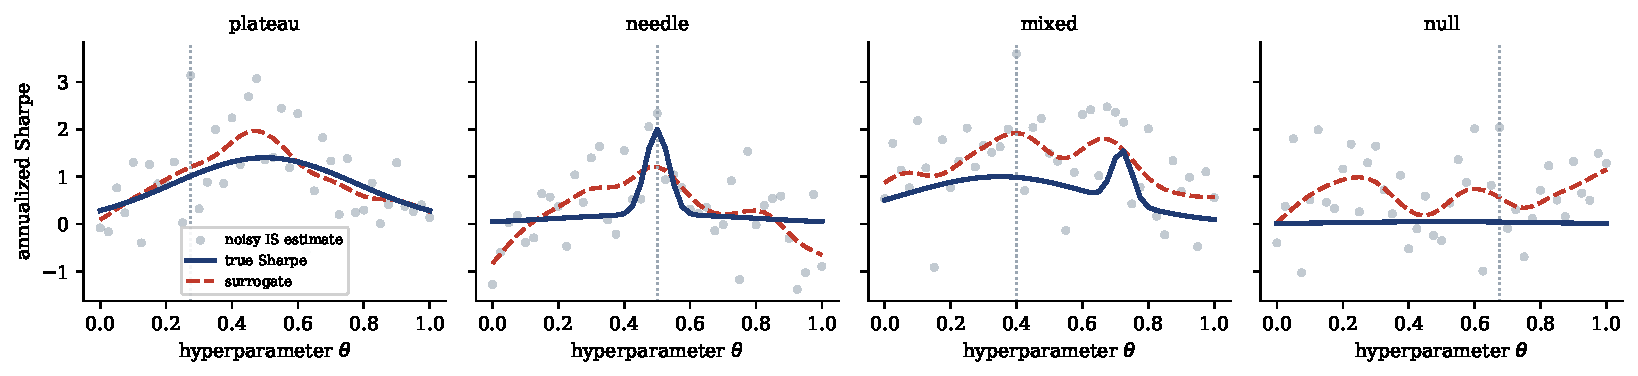
\includegraphics[width=\textwidth]{fig_setup.pdf}
\caption{The four canonical landscapes (one hyperparameter). Solid: population
Sharpe. Dots: a single noisy in-sample estimate per grid cell. Dashed: the
kernel surrogate on which plateau geometry is measured. Dotted vertical: the
naive argmax of the raw estimate. The \emph{null} panel has no real edge, yet its
smoothed surrogate still presents a benign-looking plateau---the failure mode
shape-based geometry cannot see.}
\label{fig:setup}
\end{figure}

\paragraph{Selection rules and outcomes.} The \emph{naive} rule selects the raw
argmax; the \emph{plateau-aware} rule selects the surrogate argmax, which prefers
a broad maximum over a lucky isolated spike. Because the truth is known we record,
for each experiment, the oracle configuration $\arg\max \sr_{\text{true}}$, the
\emph{true regret} $\sr_{\text{true}}(\text{oracle})-\sr_{\text{true}}(\hat\theyll)$,
the in-sample$\to$out-of-sample inflation gap, and the realized OOS Sharpe of
each rule, alongside every diagnostic.

\section{Experimental setup}
\label{sec:setup}

Each experiment samples a random landscape from one of four families---wide
\emph{plateau}, sharp \emph{needle}, \emph{mixed} (plateau plus a taller spike),
and \emph{null} (no edge)---with randomized amplitudes, widths, centers, factor
share and in-sample length, on a grid of $41^d$ configurations. We run
$N{=}5{,}000$ one-parameter and $N{=}4{,}000$ two-parameter problems. PBO uses
$S{=}10$ blocks; the plateau margin is $\delta{=}0.25$ Sharpe. The surrogate
bandwidth is $0.06$ of the axis, i.e.\ $\sigma = 2.4$ grid cells: the a-priori
rationale is that this sits well below the true plateau scales of the generator
($\ell_p \in [0.15, 0.45]$, i.e.\ $6$--$18$ cells), so the kernel averages away
cell-level noise without erasing plateau-scale structure. It was not tuned to
the results, but it is a choice, and Section~\ref{sec:selection} reports the
selection payoff across bandwidths $0.03$--$0.16$ in both dimensions, including
where it degrades.

We score each diagnostic against three ground-truth binary labels capturing
distinct overfitting modes: \textbf{no-edge}, the selected configuration has true
Sharpe below $0.25$ (deployed something essentially worthless); \textbf{fragile},
true regret exceeds $0.5$ (left real edge on the table by landing on a fragile or
wrong point); and \textbf{OOS-loss}, the selected configuration loses money out of
sample. Labels are defined for the \emph{naive} selection---the behavior the
diagnostics are meant to audit---while the plateau geometry is anchored at the
\emph{surrogate} optimum, the heuristic's own object; Section~\ref{sec:anchoring}
quantifies how much this anchoring choice matters. Discriminative power is the
ROC AUC of the (orientation-aligned) diagnostic, with $95\%$ confidence
intervals from $1{,}000$ bootstrap resamples of the experiment records;
complementarity is the cross-validated AUC of an $L_2$ logistic combination
(scaler and classifier fitted inside each fold). To verify the conclusions are
not artifacts of the label cutoffs we recompute the full AUC table with the
no-edge threshold in $\{0.15, 0.25, 0.35\}$ and the fragile threshold in
$\{0.35, 0.5, 0.65\}$: AUCs shift by at most $0.05$ ($0.07$ for the single
near-chance outlier-gap/fragile cell), and the best diagnostic for each label
never changes. All code, seeds and the exact configuration are released.

\section{Results}

\subsection{As standalone diagnostics: significance tests dominate, shape metrics do not}
\label{sec:diagnostic}

Figure~\ref{fig:auc} and Table~\ref{tab:auc} report detection AUCs. Three
findings stand out.

First, the plateau-\emph{shape} metrics are weak. In one dimension the
robustness score is at chance for the no-edge mode (AUC $0.501$) and barely
above it for fragile ($0.520$); curvature is \emph{anti}-predictive of no-edge
($0.369$), because a sharp surrogate peak indicates that \emph{some} real signal
exists---the opposite of the no-edge case. The article-style fixed thresholds
inherit this weakness: at $R>0.1$ the implied ``robust'' subset ($52\%$ of the
one-dimensional experiments) has an overfit base rate of $38.6\%$ versus
$38.5\%$ overall, so the threshold separates nothing; in two dimensions $92\%$
of experiments pass it.

Second, the strongest single diagnostic is the plain PSR against zero (no-edge
AUC $0.808$, OOS-loss $0.733$), ahead of the DSR ($0.785$, $0.713$) and PBO
($0.669$, $0.643$). The explanation is unglamorous: the no-edge label
(``selected configuration has true Sharpe below $0.25$'') is close to the PSR's
own null hypothesis, so the significance test against zero is nearly tailor-made
for it---and the DSR's multiplicity deflation adds nothing to the \emph{ranking}.
The deflation benchmark $\sr_0$ is proportional to the cross-sectional
dispersion of Sharpe estimates, which in our generator is largest exactly when a
real edge exists, so deflating partially cancels the signal. Consistently,
recomputing the DSR as if only $10\%$ of the grid trials were independent
(i.e.\ less deflation, arguably more honest given the correlated trials noted in
Section~\ref{sec:background}) slightly \emph{raises} its no-edge AUC, from
$0.785$ to $0.802$ in $d{=}1$ and from $0.735$ to $0.743$ in $d{=}2$. None of
this says the DSR is wrong---it is a calibrated significance test, and AUC
measures ranking, not calibration---but for ranking overfitting risk in this
setting the deflation term contributes no discriminative power beyond the
underlying PSR.

Third, the one genuinely informative geometry-family diagnostic is the
\emph{outlier gap} (no-edge AUC $0.703$ in $d{=}1$ and $0.837$ in
$d{=}2$---where it is the best diagnostic of any kind). Note what it measures:
whether the best cells stand far above typical performance, i.e.\ signal
\emph{amplitude} on the smoothed landscape, not shape. The practitioner intuition
that survives validation is ``check that the top of the landscape clears the
typical level,'' not ``check that the top is wide.''

\begin{figure}[t]
\centering
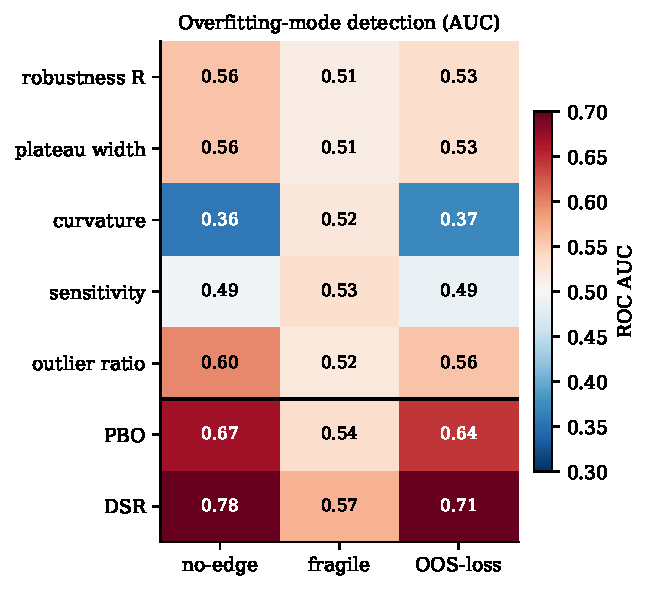
\includegraphics[width=0.62\textwidth]{fig_auc.pdf}
\caption{Detection AUC (one parameter, $N{=}5{,}000$). Rows above the line are
plateau-geometry diagnostics; below are statistical baselines. Red marks
AUC $>0.5$ (informative for that overfitting mode); blue marks AUC $<0.5$
(anti-informative). The shape metrics hover near chance; the amplitude-style
outlier gap and the significance tests carry the no-edge and OOS-loss signal.}
\label{fig:auc}
\end{figure}

\begin{table}[t]
\centering
\caption{Detection AUC by diagnostic and overfitting mode. Higher is better;
$0.5$ is chance and values below $0.5$ are anti-informative. Best in each
column in \textbf{bold}. $95\%$ bootstrap confidence-interval half-widths range
from $\pm0.014$ to $\pm0.024$ across cells. In $d{=}1$ the robustness score and
the plateau width coincide by construction (single axis, unit fANOVA weight),
so their rows are identical there.}
\label{tab:auc}
\small
\begin{tabular}{lccc@{\hskip 2em}ccc}
\toprule
& \multicolumn{3}{c}{One parameter ($d{=}1$)} & \multicolumn{3}{c}{Two parameters ($d{=}2$)}\\
\cmidrule(lr){2-4}\cmidrule(lr){5-7}
Diagnostic & no-edge & fragile & OOS-loss & no-edge & fragile & OOS-loss \\
\midrule
Robustness score $R$ & 0.501 & 0.520 & 0.483 & 0.558 & 0.585 & 0.519 \\
Plateau width        & 0.501 & 0.520 & 0.483 & 0.546 & 0.587 & 0.510 \\
Curvature            & 0.369 & 0.528 & 0.380 & 0.431 & \textbf{0.635} & 0.449 \\
Outlier gap          & 0.703 & 0.481 & 0.655 & \textbf{0.837} & 0.478 & \textbf{0.719} \\
\midrule
PBO                  & 0.669 & 0.535 & 0.643 & 0.727 & 0.585 & 0.670 \\
DSR                  & 0.785 & \textbf{0.570} & 0.713 & 0.735 & 0.573 & 0.656 \\
PSR                  & \textbf{0.808} & 0.560 & \textbf{0.733} & 0.759 & 0.580 & 0.669 \\
\bottomrule
\end{tabular}
\end{table}

\subsection{Where combining geometry with statistics helps---and where it does not}
\label{sec:complementarity}

The two families specialize. Statistical diagnostics excel at the \emph{no-edge}
mode---selecting from pure noise---which is what they were built for. Plateau
geometry, by construction, sees the \emph{shape} of the optimum and contributes
on the \emph{fragile} mode, but is blind to no-edge: a flat null surface smooths
into a wide, benign-looking plateau (Figure~\ref{fig:setup}, rightmost panel).
The risk-oriented diagnostics are only weakly correlated across families
(Spearman $|\rho|\le 0.28$ between $R$ and PBO/DSR/PSR in $d{=}1$), so there is
information to combine---but the bootstrap confidence intervals show the gain is
conditional, not universal (Figure~\ref{fig:comp}).

In one dimension, the logistic combination of geometry and statistics
($R$, curvature, PBO, DSR) significantly improves on the DSR for no-edge
($\Delta\mathrm{AUC} = +0.017$, $95\%$ CI $[+0.008, +0.026]$) and OOS-loss
($+0.022$, $[+0.011, +0.034]$), but \emph{not} for fragile ($+0.001$,
$[-0.010, +0.012]$). Against the plain PSR the combination adds nothing
significant on no-edge ($-0.000$, $[-0.010, +0.009]$; both reach AUC $0.801$
vs.\ $0.801$) or OOS-loss ($+0.011$, $[-0.001, +0.023]$); it wins only on
fragile ($+0.072$, $[+0.050, +0.094]$), where the PSR is at chance. In two
dimensions the picture is cleaner: the combination significantly beats every
single diagnostic in its feature set on every label (vs.\ DSR: $+0.039$
no-edge, $+0.093$ fragile, $+0.037$ OOS-loss; all intervals exclude zero),
reaching AUC $0.774$/$0.664$/$0.692$. One honest caveat: the feature set was
fixed in advance to the folklore comparison (shape metrics $+$ PBO $+$ DSR), and
in $d{=}2$ the outlier gap \emph{alone} (AUC $0.837$) beats this combination on
no-edge---so the combination numbers understate what a fuller model could do,
and we report them as a test of the ``shape complements statistics'' claim, not
as a best-possible detector.

\begin{figure}[t]
\centering
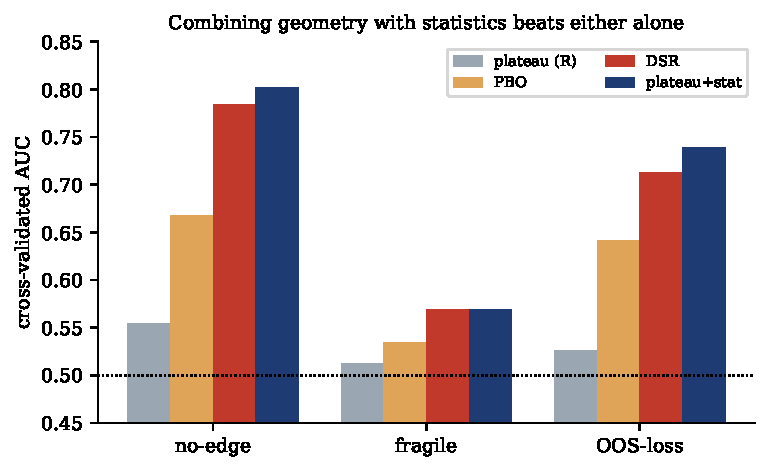
\includegraphics[width=0.7\textwidth]{fig_complementarity.pdf}
\caption{Cross-validated AUC of single diagnostics versus a logistic combination
of plateau and statistical features (one parameter; error bars are $95\%$
bootstrap confidence intervals). The combination significantly improves on the
DSR for no-edge and OOS-loss but not for fragile, and is statistically
indistinguishable from the plain PSR everywhere except the fragile mode, where
the PSR is at chance.}
\label{fig:comp}
\end{figure}

\subsection{Dimensionality helps the geometry, with a caveat}
\label{sec:dimension}

The right half of Table~\ref{tab:auc} repeats the analysis with two
hyperparameters. Overfitting is worse---base rates of every failure mode
rise---and the geometry gains traction: the robustness score's no-edge AUC rises
from $0.501$ to $0.558$ and its fragile AUC from $0.520$ to $0.585$; curvature
becomes the single best fragile detector ($0.635$); and the amplitude-style
outlier gap strengthens most ($0.703 \to 0.837$), overtaking every statistical
diagnostic for no-edge and OOS-loss detection. The significance tests weaken
slightly (PSR $0.808 \to 0.759$) as the grid grows from $41$ to $1{,}681$
correlated trials. The combined classifier's advantage over the best single
statistical diagnostic widens accordingly (Section~\ref{sec:complementarity}),
and the fragile mode---where shape information lives---is detected at $0.664$
versus at most $0.585$ for any statistical diagnostic alone. The caveat: even in
$d{=}2$ the shape metrics on their own remain modest ($0.5$--$0.6$); what grows
with dimensionality is their \emph{marginal} value in combination, and the
amplitude signal, not standalone shape-based detection.

\subsection{Anchoring matters: geometry inverts at the naive optimum}
\label{sec:anchoring}

The plateau geometry above is measured at the surrogate's own argmax, while the
labels describe the naive selection. This is the heuristic's intended use
(assess the denoised landscape, then act on it), but it is a choice, and we
quantify it: every experiment also records the same metrics anchored at the
\emph{naive} argmax on the same surrogate. Anchored there, the geometry
inverts: the robustness score's no-edge AUC falls from $0.501$ to $0.418$ in one
dimension and from $0.558$ to $0.203$ in two---decisively anti-informative. The
mechanism is instructive. On a no-edge landscape the surrogate around the
noise-selected point is flat, so naive-anchored geometry reports a wide, benign
plateau precisely when the selection is pure luck; when a real edge exists the
surrogate has structure and the same metrics report more fragility. Plateau
geometry is a property of the denoised landscape at its own optimum, not of
whatever point the optimizer returned; practitioners who compute plateau metrics
around the raw optimizer output---the most natural implementation---should
expect the inverted behavior.

\subsection{As a selection rule, ``prefer plateaus'' works}
\label{sec:selection}

The practical question is not only whether geometry diagnoses overfitting but
whether \emph{acting} on it helps. Table~\ref{tab:selection} and
Figure~\ref{fig:selection} compare the naive and plateau-aware selection rules
out of sample. Preferring the surrogate optimum raises mean OOS Sharpe from
$1.12$ to $1.24$ in one dimension ($+0.115$; Wilcoxon
$p \approx 7\times10^{-19}$) and from $0.86$ to $1.17$ in two ($+0.307$;
$p \approx 4\times10^{-71}$). In $d{=}1$ the two rules pick the same cell in
$21\%$ of experiments; among non-ties the plateau-aware rule wins $56\%$ of the
time with a median gain of $+0.144$. The gain rises monotonically with the
curvature of the surrogate at its optimum: $+0.062$ in the flattest tercile
(one-sample $t$-test $p = 0.005$), $+0.107$ in the middle, $+0.177$ in the
sharpest for $d{=}1$; and $+0.091$/$+0.257$/$+0.575$ for $d{=}2$ (all
$p < 10^{-3}$). The rule is targeted insurance against the sharp-peak failure
mode, and on these landscapes the insurance costs nothing: even in the
smoothest tercile, where it should be least needed, the expected payoff is
small but positive rather than zero.

Two qualifications keep this honest. First, the baseline is the weakest
defensible one---the raw argmax of an unsmoothed noisy surface---so the result
demonstrates the value of \emph{denoised selection}, of which ``prefer
plateaus'' is one instance, not superiority over any sophisticated alternative.
Second, the magnitude depends on the surrogate bandwidth
(Figure~\ref{fig:selection}, right). In $d{=}1$ the mean gain is $+0.100$,
$+0.106$, and $+0.089$ at bandwidths $0.045$, $0.06$, and $0.075$, decays to
$+0.040$ at $0.09$ and $+0.017$ at $0.12$, and turns negative ($-0.041$) at
$0.16$, where smoothing erases real structure; the sign flips at roughly $0.14$
of the axis. In $d{=}2$ the gain is positive across the entire tested range
(from $+0.381$ at bandwidth $0.045$ to $+0.151$ at $0.16$). Finally, an
implementation note: an earlier version of our surrogate used
boundary-replicating padding, which inflates noise variance at the grid edges
and piles the ``robust'' selection onto boundary cells of flat landscapes;
fixing this (mask-normalized smoothing, Section~\ref{sec:framework}) raised the
mean gains and made the flattest-tercile payoff positive. Geometry heuristics
inherit the artifacts of the smoother they are computed on.

\begin{table}[t]
\centering
\caption{Out-of-sample Sharpe of naive vs.\ plateau-aware selection. Ties are
experiments where both rules select the same grid cell; tercile rows split
experiments by the curvature of the surrogate at its optimum. All tercile gains
differ from zero at $p \le 0.005$ (one-sample $t$-tests).}
\label{tab:selection}
\small
\begin{tabular}{lcc}
\toprule
 & One parameter & Two parameters \\
\midrule
Naive argmax (mean OOS Sharpe)        & 1.123 & 0.862 \\
Plateau-aware (mean OOS Sharpe)       & 1.238 & 1.170 \\
Mean gain                             & $+0.115$ & $+0.307$ \\
Median gain (non-tie pairs)           & $+0.144$ & $+0.280$ \\
Win rate / ties / non-tie win rate    & 0.44 / 0.21 / 0.56 & 0.59 / 0.04 / 0.61 \\
Gain, low-curvature tercile           & $+0.062$ & $+0.091$ \\
Gain, mid-curvature tercile           & $+0.107$ & $+0.257$ \\
Gain, high-curvature tercile          & $+0.177$ & $+0.575$ \\
\bottomrule
\end{tabular}
\end{table}

\begin{figure}[t]
\centering
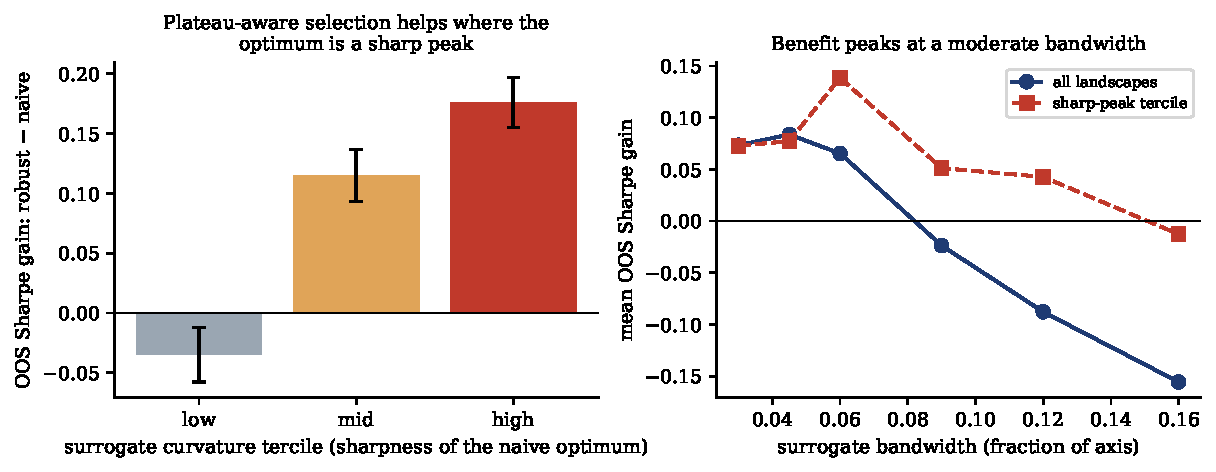
\includegraphics[width=\textwidth]{fig_selection.pdf}
\caption{Out-of-sample gain of plateau-aware over naive selection (one
parameter). Left: gain by tercile of the surrogate curvature \emph{at the
surrogate optimum} (error bars: standard errors)---the gain is positive in every
tercile and largest where that optimum is a sharp peak. Right: the gain versus
surrogate bandwidth; a moderate bandwidth is best, and over-smoothing eventually
turns the average gain negative in one dimension.}
\label{fig:selection}
\end{figure}

\section{Discussion}

The results reconcile two views that are usually stated as competitors, but not
in the way the folklore expects. The statistical school treats overfitting as a
multiple-testing problem; the geometric school treats it as a fragility problem
and inspects the shape of the optimum. Three honest lessons emerge. First, for
\emph{detecting} a worthless selection, the workhorse is the plain significance
test: the PSR against zero is the strongest single diagnostic here, and the
DSR's multiplicity deflation---with trials as correlated as a grid
scan---contributes calibration, not ranking power. Second, the plateau
heuristic's \emph{shape} metrics and rule-of-thumb thresholds are weak or
uncalibrated as standalone tests, and become actively misleading if anchored at
the raw optimizer output; what survives of the diagnostic intuition is the
amplitude check (does the top of the denoised landscape clear the typical
level?) and a complementary contribution on the fragile mode, mainly in higher
dimension. Third, the heuristic's \emph{action}---select the optimum of a
denoised landscape rather than the raw argmax---is the clearest win: a real,
monotone-in-sharpness out-of-sample improvement that grows with the number of
parameters. ``Prefer plateaus'' is best understood not as a test but as a
regularizer on selection.

\section{Limitations}

Our generative model uses Gaussian, serially independent returns with a single
shared factor; real returns have fat tails, volatility clustering, regime
shifts, and richer dependence that all amplify overfitting and may change the
relative ranking of diagnostics. We model the optimizer as exhaustive grid
evaluation plus a fixed-bandwidth smoothing surrogate; an adaptive sampler
(e.g.\ TPE or Gaussian processes) explores unevenly and would interact with the
geometry metrics differently. The labels and thresholds, while
ground-truth-based, involve choices ($\delta$, the surrogate bandwidth, the
label cutoffs); we stated the a-priori rationale for the bandwidth, showed the
AUC conclusions are stable across label cutoffs (Section~\ref{sec:setup}), and
reported rather than hid the bandwidth dependence of the selection gain,
including the sign change near $0.14$ of the axis in one dimension. The DSR is
computed with $N$ equal to the full grid size despite correlated trials; the
$N_{\text{eff}}$ sensitivity check (Section~\ref{sec:diagnostic}) suggests this
does not drive the comparison. Finally, we study Sharpe-based selection on a
single asset; portfolio-level and turnover/cost-aware objectives are left to
future work.

\section{Conclusion}

We gave the plateau-versus-peak heuristic of trading-strategy optimization its
first controlled validation against ground truth and against the standard
backtest-overfitting diagnostics. As standalone overfitting tests, the local
plateau-\emph{shape} metrics are weak, their popular fixed thresholds are not
calibrated, and the strongest single diagnostic is the plain probabilistic
Sharpe ratio against zero---the significance test, not the multiplicity
deflation, carries the detection signal in this setting. Geometry contributes
where shape information exists: the (re-posed) outlier gap is the best no-edge
detector in two dimensions, and combining shape metrics with statistical
diagnostics significantly improves fragile-mode detection. Acting on the
geometry---selecting the optimum of the denoised landscape rather than the raw
argmax---delivers a real, targeted out-of-sample improvement that is positive in
every curvature tercile and grows with dimensionality. Prefer plateaus as a
selection bias; do not rely on them as a test; and pair them with a significance
test, which sees the failure mode that shape cannot.

\paragraph{Reproducibility.} All experiments are deterministic given the
released seeds. A single command (\texttt{python scripts/run\_all.py})
regenerates every number---including the bootstrap confidence intervals and
sensitivity checks---and \texttt{python -m plateau\_experiments.figures}
regenerates every figure; a companion script
(\texttt{scripts/check\_paper\_numbers.py}) asserts that every value quoted in
this paper's tables and text matches the generated results. The implementation
of the metrics, the PBO/CSCV, PSR and DSR baselines, and the simulation is
provided as an open-source package.

\small
\bibliographystyle{plainnat}
\bibliography{refs}

\end{document}
